
\chapter{Methodology}

\section{Research context}

Swarmia is a Software as a Service tool for software development teams. Teams utilize Swarmia to measure their performance and find potential places of improvement in their development pipeline. Swarmia is designed to help teams work in a self-managed manner. 

To provide insight to the client teams, Swarmia integrates with issue trackers like Jira and version control systems like GitHub. The teams are then provided with insights that is accessible to all team members through Swarmia web application. In addition, Swarmia can be configured to push updates to the teams Slack channel. 

Swarmia can be used by a team of any size. The teams include both teams working within software companies in addition to in-house development teams of non-software companies. 

The data collected by Swarmia includes pull requests, git commits, automated test runs and issues. Furthermore, Swarmia has read-access to the source code, which is used to estimate the complexity of the change in question. Swarmia never stores the source code, but rather calculates the size of the change bundle and stores it in a distinct database. 

One of the features in Swarmia is called Working Agreements. Teams can configure up to 8 of these agreements, which could more generally be described as "team norms" or "collaboration guidelines". The agreements are be selected from predefined list of options, but each team can customise them to suit their use case. For example, a team could agree that they want to enforce linking pull requests to issues. Swarmia would then track the set condition automatically and inform the teams about the status of the agreement. 

Working agreement options in Swarmia are presented in Figure \ref{fig:WorkingAgreements}.

\begin{table}[h!]
\centering
\begin{tabular}{ |c|c| } 
\hline
option in Swarmia & computer readable \\ [0.5ex] 
\hline\hline
Avoid pushing directly to the default branch & no\_direct\_pushes\_to\_main\_branch \\
Avoid working alone & min\_issue\_contributors  \\
Limit issues in progress & wip\_issues  \\
Limit pull requests in progress & wip\_pull\_requests \\
Link pull requests to issues & pull\_request\_linking  \\
Reduce issue cycle time & max\_issue\_age  \\
Reduce pull request cycle time & max\_pull\_request\_age \\
Reduce pull request review time & max\_pull\_request\_review\_time  \\
\hline
\end{tabular}
\caption{Working Agreement options}
\label{tab:workingAgreements}
\end{table}

- connection to the scientific background: DORA, some papers
- table with human readable wa name and the backend slug

\begin{figure}[ht]
    \begin{center}
        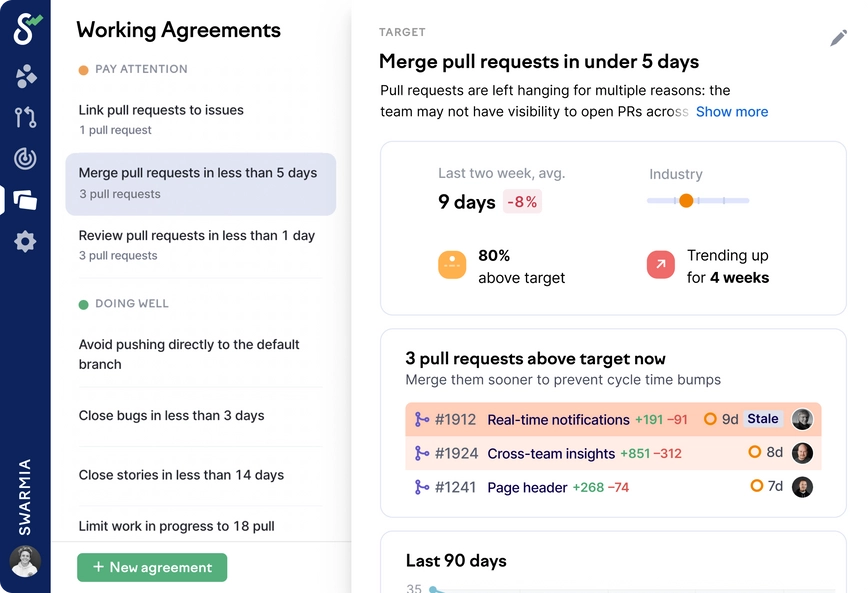
\includegraphics[width=13.5cm]{LaTeX/images/improvement.png}
        \caption{Working Agreements in Swarmia}
        \label{fig:WorkingAgreements}
    \end{center}
\end{figure}

\section{Research questions}

The main research question of this thesis is to look into how teams use Working Agreements: which share of Swarmia teams use the feature and how these teams have configured their Working Agreements setup. 

The second research question is to find out if Working Agreements can enhance productivity in software development teams. The hypothesis based on previous research is that as Working Agreements promote methods that are shown to accelerate software development, they should have direct impact on the team's productivity. We are going to look into the Working Agreement composition in different teams and find out which of the agreements have the most impact on the teams performance. 

\section{Approach}

To answer RQ1, data from Swarmia is used to determine how many of the teams have enabled which Working Agreements. Furthermore, we look into how many Working Agreements teams usually have in use and what kind of parameters they have configured in Swarmia: for example, what is their WIP limit in \textit{Limit issues in progress} agreement? Lastly, team characteristics such as team size and their connection to Working Agreements setup is analysed. The RQ1 is approached with simple SQL queries. 

To answer RQ2, data of all teams using Working Agreements feature is collected and analyzed. Historical activity data is pulled from the teams' source control repositories. The data is aggregated weekly for 24-month period: some teams have been clients for longer than 2 years and some for shorter amount. This should not be a problem, as averages are used and the data collection period itself is not a variable in the analysis.

The key metric to be used in the analysis is the Pull Request Cycle Time (PRCT). Even though Swarmia exports data also from issue trackers, these data sources were left out of the analysis based on the scope of the thesis.

The analysis is done in Google's BigQuery data warehouse in line with Swarmia's data handling policy. In addition to standard SQL queries, BigQuery has machine learning capabilities. For this thesis, the inbuilt linear regression feature was utilized. The data flow before building the regression model is presented in Figure \ref{fig:dataFlow}. 

The training data is passed to linear regression in a form presented in Table \ref{table:trainingDataStructure}. The data has gone through two major modifications to better fit for the model. First, we have calculated an average PRCT for each team from the time before they have enabled any working agreements. This average is then subtracted from each rows PRCT to achieve normalized dataset: the aim is to diminish the differences between teams to achieve comparable PRCTs. Secondly, WA activation dates are mapped to 0/1 boolean values for each row: the value is 0 if WA has not been activated yet and 1 if it has.

\begin{table}
\begin{center}
\begin{tabularx}{\textwidth}{ |l|X| } 
\hline
parameter & description \\ [0.5ex] 
\hline\hline
wip\_pull\_requests & WA status \\
max\_pull\_request\_age & WA status \\
no\_direct\_pushes\_to\_main\_branch & WA status \\
min\_issue\_contributors  & WA status \\
wip\_issues & WA status \\
max\_issue\_age  & WA status \\
max\_pull\_request\_review\_time  & WA status \\
pull\_request\_linking  & WA status \\
ct\_days  & normalized cycle time in days \\
github\_authors & Pull request authors \\
swarmia\_users & MAU in Swarmia team \\
slack\_users & Swarmia users with Slack notifications \\
daily\_digest & team's Slack daily digest status \\
\hline
\end{tabularx}
\caption{Linear regression training data structure}
\label{tab:trainingDataStructure}
\end{center}
\end{table}




\begin{figure}[ht]
\centering
\begin{tikzpicture}[
    every node/.style={align=center, minimum height=1em, minimum width=1cm,node distance=0.7cm},
]

%Nodes
\node[entity]      (teamswa)        {active teams with WA adoption};
\node[entity]      (teams)          [above=of teamswa] {team basic info};
\node[entity]      (snapshots)       [left=of teams] {team snapshots};
\node[entity]       (mau)           [right=of teams] {MAU};
\node[entity]      (ctwa)       [below=of teamswa] {cycle times with WA adoption};
\node[entity]      (cycletimes)       [left=of ctwa]     {cycle times};
\node[entity]      (adoption)       [left=of snapshots] {WA adoption};
\node[entity, fill=gray!20]       (lm)        [below=of ctwa] {linear model input data};

%Lines
\draw[->] (cycletimes.east) -- (ctwa.west);
\draw[->] (ctwa.south) -- (lm.north);
\draw[->] (teamswa.south) -- (ctwa.north);
\draw[->] (teams.south) -- (teamswa.north);
\draw[->] (snapshots.south) -- (teamswa.north);
\draw[->] (mau.south) -- (teamswa.north);
\draw[->] (adoption.south) -- (teamswa.north);

\end{tikzpicture}
\caption{Data flow in BigQuery}
\label{fig:dataFlow}
\end{figure}

\section{Results}

\subsection{RQ1 results}

To get an overview on how teams are using Working Agreements, we started with the proportional popularity of WAs. As can be seen in Figure \ref{fig:waPopularity}, the agreements max\_pull\_request\_review\_time and max\_pull\_request\_age are the used the most, with over three hundred teams using them. Another atypical WA is min\_issue\_contributors, with approximately only 150 teams using.

\begin{filecontents}{usage.data}
type amount
1 206 
2 225
3 315
4 229
5 148
6 204
7 219
8 341
9 111
\end{filecontents}

\begin{figure}[h!]
\centering
\begin{tikzpicture}
\begin{axis}[
	x tick label style={
		 rotate=45, anchor=east},
	ylabel=Number of teams using,
        xticklabels={\texttt{\detokenize{pull_request_linking}},\texttt{\detokenize{max_issue_age}},\texttt{\detokenize{max_pull_request_age}},\texttt{\detokenize{no_direct_pushes_to_main_branch}},\texttt{\detokenize{min_issue_contributors}},\texttt{\detokenize{wip_issues}},\texttt{\detokenize{wip_pull_requests}},\texttt{\detokenize{max_pull_request_review_time}}},
	enlargelimits=0.05,
	legend style={at={(0.5,-0.1)},
	anchor=north,legend columns=-1},
	ybar interval=0.8,
        ymin=0
]
\addplot[fill=cyan] table[x=type, y=amount] {usage.data};
\end{axis}
\end{tikzpicture}
\caption{Working Agreement usage}
\label{fig:waPopularity}
\end{figure}

A distribution of how many WAs each team has in use was calculated. The results are plotted in Figure \ref{fig:waDistribution}. Even though there exists eight Working Agreement templates, the number of WAs in use can exceed this: some templates can be configured multiple times for a single team. For example, max\_issue\_age can be configured distinctly for epics, stories, tasks and bugs. Still, only a small share of teams have configured more than eight WAs. 

\begin{filecontents}{wa.data}
was teams
1 23.55
2 15.08
3 13.64
4 11.36
5 12.60
6 6.82
7 7.02
8 5.58
9 1.65
10 1.24
11 0.62
12 0.62
13 0.21
14 1
\end{filecontents}

\begin{figure}
\centering
\begin{tikzpicture}
\begin{axis}[
	x tick label style={
		/pgf/number format/1000 sep=},
	ylabel=Percentage of teams,
        xlabel=Amount of WAs,
	enlargelimits=0.05,
	legend style={at={(0.5,-0.1)},
	anchor=north,legend columns=-1},
        yticklabel={\pgfmathparse{\tick}\pgfmathprintnumber{\pgfmathresult}\%},
	ybar interval=0.8,
]
\addplot[fill=cyan] table[x=was, y=teams] {wa.data};
\end{axis}
\end{tikzpicture}
\caption{Teams' WA usage distribution}
\label{fig:waDistribution}
\end{figure}

\subsection{RQ2 results}











